\documentclass[12pt,titlepage]{article}





%PACKAGES
\usepackage[ngerman]{babel}
\usepackage[utf8]{inputenc}
\usepackage[a4paper,lmargin={2.5cm},rmargin={2.5cm},
tmargin={2.5cm},bmargin = {2.5cm}]{geometry}
\usepackage{graphicx}
\usepackage{caption}
\usepackage{float}
\usepackage{hyperref}
\parindent0pt





\begin{document}



\thispagestyle{empty}

%TITELSEITE
\begin{center}
\textbf{Hochschule Luzern}\\
Departement für Informatik\\[12\baselineskip]

\begin{Huge}
Projekt FoodPrint
\end{Huge} \\[6\baselineskip]

\begin{large}
\textbf{Programmieren fürs iOS}
\end{large} \\[6\baselineskip]

\begin{large}
\textbf{Studierende}: Frederico Fischer, Nico Iseli\\
\textbf{Dozenten}: Prof. Dr. Ruedi Arnold, Nicolas Märki\

\textbf{Abgabedatum}: 13. Dezember 2020 \\[3\baselineskip]

\begin{figure}[ht]
  \centering
  \begin{minipage}[t][][b]{0.2\textwidth}
  \href{https://github.com/NicoIseli/IOS_App_Project}{
\includegraphics[width=\textwidth]{Img/iosappqrcode.png}}
    \caption*{iOS-App}
  \end{minipage}
  \hfill
  \begin{minipage}[t][][b]{0.2\textwidth}
    \href{https://gitlab.enterpriselab.ch/foodprint/foodprint-backend-distribution}{
\includegraphics[width=\textwidth]{Img/backendqrcode.png}}
    \caption*{Webservice}
  \end{minipage}
\end{figure}
\end{large}
\end{center}
\newpage


\section{Einleitung}
Das vorliegende Projekt hat zum Ziel, eine App zu entwickeln, um Menschen mehr zu unweltfreundlichen Einkäufen zu ermutigen. Die App soll dabei bedürfnisbasiert regionale und saisonale Produkte vorschlagen. Die Implementierung ist vorerst für Benutzer aus der Schweiz vorgesehen. Das Datenbankschema im Backend ist jedoch so aufgebaut, dass sich die App auch auf weitere Länder erweitern lässt.

\section{Architektur}
Die Architektur ist so aufgebaut, dass die benötigten Produktdaten über eine REST-API zur Verfügung gestellt werden. Die Produktdaten werden über HTTP-Requests geladen und auf der App mittels Core-Data persistiert, wobei die Daten auch gleich abgeglichen werden. Neben den Produktdaten werden die User-Einstellungen ebenfalls mittels Core-Data persistiert, wobei man diese nur App-Intern verwaltet. Die User-Daten werden genutzt, um die Produkte userspezifisch zu filtern. Das User-Interface wurde mit dem UI-Kit aufgebaut. Die Architektur ist als Abbildung (vgl. Abbildung \ref{img: Architektur} auf Seite \pageref{img: Architektur}) festgehalten.
\begin{figure}[H]
	\centering
	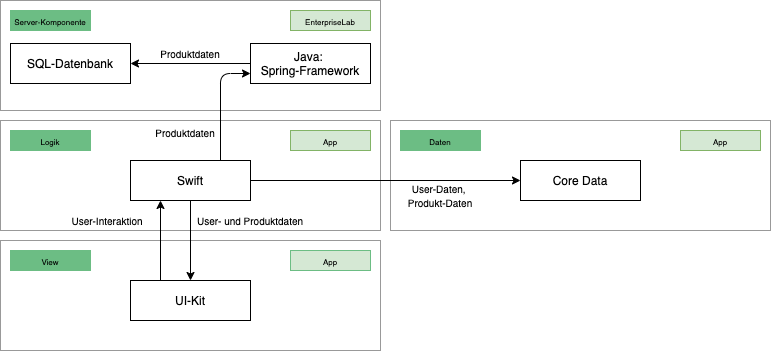
\includegraphics[width=15cm]{Img/Architektur2.png}
	\caption[Architektur]{Architektur,\\ Quelle: Projektteam}
	\label{img: Architektur}
\end{figure}

\section{Feature-List}
\begin{itemize}
	\item \textbf{User-Settings:} Bedürfnisorientierte Einstellungen, wie die Produkte gefiltert werden sollen
	\item \textbf{Userspezifische Produktauflistung:} Auflistung der gefilterten Produktdaten gemäss den User-Einstellungen
	\item \textbf{Produkt-Details:} Detail-View für jedes Produkt, in der ein vertiefterer Einblick möglich ist
	\item \textbf{About-View:} View mit Informationen über die Intention und Funktionsweise der App
\end{itemize}

\section{Umsetzung technischer Anforderungen}
\subsection{Server-Komponente} \label{Server-Komponente}
Für die Server-Komponente wird eine Ressource im EnterpriseLab verwendet. Als Datenbank verwendet man MariaDb und als Java-Framework greift man auf SpringBoot zurück. Die Anbindung der Datenbank zum SpringBoot wurde mittels der JPA-Schnittstelle (OR-Mapper) umgesetzt. Bei der Datenbank wurde Wert darauf gelegt, ein erweiterbares Schema zu definieren, da eine Weiterentwicklung der Applikation geplant ist. Über einen REST-Controller werden die Produktdaten dann im JSON-Format zurückgegeben (ersichtlich unter: \url{http://ffischer-ios-h20.el.eee.intern:8080/api/v1/products/Schweiz}). Aktuell läuft der Server nicht in der DMZ. Daher ist ein Aufruf nur mit bestehender VPN-Verbindung im HSLU-Netzwerk möglich.\\
\\
\textbf{Code-Referenz: }\path{foodprint-backend-distribution}

\subsection{HTTP-Kommunikation}
Die JSON-Daten des Webservers werden über den Aufruf der  URL (vgl. Abschnitt \ref{Server-Komponente} auf Seite \pageref{Server-Komponente}) geladen und mittels des JSON-Decoders von Swift in ein Array von Swift-Objekten konvertiert. Dabei wird mit Data Transfer Objects (DTO) gearbeitet, die während der Konzipierung der API definiert wurden.\\
\\
\textbf{Code-Referenz: }\\ \path{FoodPrint/ FoodPrint/ViewControllers/ProductListViewController.swift} \\ In diesem File ist der entsprechende Code unter dem Abschnitt \textbf{\glqq MARK: - API\grqq\,} ersichtlich.

\subsection{Persistierung mit Core-Data}
Mittels Core-Data werden die User-Daten sowie die Produktdaten lokal persistiert. Die Produktdaten werden vor der Persistierung noch mit einer entsprechenden Logik verarbeitet, da die geholten DTO's noch nicht dem entsprechen, was im User-Interface schlussendlich angezeigt werden soll. Die App verwaltet dabei ingesamt einen User und mehrere Produktdaten. Diese können gelesen (über die Fetch-Methode im NSManagedContext) und persistiert (über die Save-Methode im NSManagedContext) werden. Der persistierte User dient dazu, die Bedürfnisse zu ändern und demzufolge die entsprechenden Produktdaten zu filtern. Während die Produktdaten im Core-Data persistiert werden, wird die Filterung In-Memory vorgenommen.\\
\\
\textbf{Code-Referenz: }\\ \path{FoodPrint / FoodPrint / Utils / CoreData.swift}

\subsection{Unit-Tests}
Unit-Tests kamen insbesondere bei der Logik zur Anwendung. Damit die Daten richtig gefiltert werden, war es wichtig, verschiedene Fälle zu berücksichtigen. Daher versuchte man, möglichst alle Ausnahmefälle zu evaluieren und somit verschiedene Tests für die unterschiedlichen Funktionen durchzuführen.\\
\\
\textbf{Code-Referenz: }\\ \path{FoodPrint / FoodPrintTests / FoodPrintTests.swift}

\subsection{Auto-Layout}
Für das Projekt wurden die verschiedenen Inhalte der einzelnen View-Controller mittels Auto-Layout formatiert. Dafür wurden entsprechende Constraints gesetzt. Die Nutzung dieses Features wurde jedoch zu wenig gut geplant. Dieses wurde ohne grosses Vorwissen genutzt, was dazu führte, dass die Constraints mehrmals gelöscht und wieder neu erstellt werden mussten. Zudem wurden auch zu wenig Geräte getestet. Aktuell sieht die Formatierung auf neueren beziehungsweise grösseren Geräten gut aus. Hingegen auf kleineren Geräten (beispielsweise auf dem I Phone SE) überlappen sich einige Inhalte. Um dies zu beheben, wurde versucht, im Nachhinein noch eine Scroll-View zu integrieren. Diese kam dann jedoch mit den bestehenden Constraints in Konflikt. Daher ist die App aktuell nicht auf alle Geräte ausgelegt.\\
\\
\textbf{Code-Referenz: }\\ \path{FoodPrint/FoodPrint/Utils/Main.storyboard}

\section*{Erkenntnisse}
Das Erstellen einer eigenen App war eine sehr interessante Erfahrung. Das Wissen über die iOS-Plattform sowie die Programmiersprache \glqq Swift\grqq{} hat sich im Team durch das Projekt stark verbessert. Während der Entwicklung sind viele kleine Fehler als auch architektonische Probleme aufgetaucht, ohne die man im Nachhinein sicherlich effizienter gewesen wäre. Ein Beispiel dafür ist die Nutzung vom Auto-Layout. Ein Problem dabei war es, dass zu schnell damit begonnen wurde. Es mussten immer wieder Constraints gelöscht und neu erstellt werden. Ein anderes Beispiel ist das Datenmanagement. Hier wurden die bisherigen Produktdaten von Hand abgetragen, weil keine passenden Quellen gefunden wurden. Kämen neue Produkte dazu, müsste die Datenerhebung überdacht werden. Eine weitere Hürde war auch das Aufsetzen der Logik. Diese wurde unterschätzt. Beim Filtern der Daten gab es diverse Ausnahmefälle, die betrachtet werden mussten. Dazu gehört beispielsweise die Auseinandersetzung mit den Saisonzeiten der Produkte. Einerseits wurde anfangs nicht berücksichtigt, dass man dieses Array auch unsortiert erhalten könnte. Andererseits musste die Kalkulation der Saison mehrmals getestet werden, da der Übergang vom Dezember zum Januar ein spezieller Fall ist. Zuletzt war die Persistierung der Produktdaten ebenfalls eine Herausforderung. Damit die Daten der API in der App nicht jedesmal neu persistiert werden, wurde eine entsprechende Überprüfung eingebaut. Aktuell ist es so, dass effektiv jedes Produkt nach deren Existenz in Core-Data überprüft wird. Dies könnte man effizienter lösen, in dem man beispielsweise mit Hashes auf der Serverseite arbeitet. Abgesehen davon ist man aber mit dem Resultat sehr zufrieden und motviert, die App auch im Anschluss an die Projektabgabe weiterzuführen.










\end{document}